\chapter{Fonctions de deux variables réelles}

\minitoc

Dans tout le chapitre, on note \(\norme{\cdot}\) la norme euclidienne canonique de \(\R^2\), \cad la norme associée au produit scalaire canonique \(\ps{\cdot}{\cdot}\) de \(\R^2\) : \[\quantifs{\forall x,y\in\R^2}\norme{\paren{x,y}}=\sqrt{x^2+y^2}.\]

\section{Ouverts de \(\R^2\)}

\begin{defi}[Boules]
Soient \(a=\paren{a_1,a_2}\in\R^2\) et \(r\in\Rp\).

La boule ouverte de centre \(a\) et de rayon \(r\) est l'ensemble des points \(x\) dont la distance à \(a\) est strictement inférieure à \(r\) : \[\bouleo{a}{r}=\accol{x\in\R^2\tq\norme{a-x}<r}.\]

La boule fermée de centre \(a\) et de rayon \(r\) est l'ensemble des points \(x\) dont la distance à \(a\) est inférieure à \(r\) : \[\boulef{a}{r}=\accol{x\in\R^2\tq\norme{a-x}\leq r}.\]

La sphère de centre \(a\) et de rayon \(r\) est l'ensemble des points \(x\) dont la distance à \(a\) est égale à \(r\) : \[\sphere{a}{r}=\accol{x\in\R^2\tq\norme{a-x}=r}.\]

Les notations \(\bouleo{a}{r}\), \(\boulef{a}{r}\) et \(\sphere{a}{r}\) ne sont pas \guillemets{officielles}.
\end{defi}

\begin{defi}
Soient \(a\in\R^2\) et \(V\subset\R^2\).

On dit que \(V\) est un voisinage de \(a\) dans \(\R^2\) s'il contient une boule centrée en \(a\) et de rayon strictement positif : \[\quantifs{\exists\epsilon\in\Rps}\bouleo{a}{\epsilon}\subset V.\]
\end{defi}

\begin{defi}[Ouvert]
Soit \(\Omega\subset\R^2\).

On dit que \(\Omega\) est un ouvert de \(\R^2\) (ou une partie ouverte de \(\R^2\)) si \(\Omega\) est un voisinage de chacun de ses points, \cad : \[\quantifs{\forall a\in\Omega;\exists\epsilon\in\Rps}\bouleo{a}{\epsilon}\subset\Omega.\]
\end{defi}

\begin{exoex}
Parmi les parties de \(\R^2\) suivantes, lesquelles sont des ouverts ?

\[\ensvide\qquad\R^2\qquad\paren{\Rps}^2\qquad\paren{\Rp}^2\qquad\R^2\excluant\accol{\paren{0,0}}\qquad\paren{\Rs}^2\qquad\intervei{0}{1}\times\R\qquad\intervee{0}{1}\times\R\]
\end{exoex}

\begin{corr}
\(\ensvide\) est un ouvert.

\(\R^2\) est un ouvert car \(\quantifs{\forall a\in\R^2}\bouleo{a}{1}\subset\R^2\).

\(\paren{\Rps}^2\) est un ouvert car \(\quantifs{\forall\paren{x,y}\in\R^2}\bouleo{\paren{x,y}}{\min\accol{\abs{x};\abs{y}}}\subset\paren{\Rps}^2\).

\(\paren{\Rp}^2\) n'est pas un ouvert.

\(\R^2\excluant\accol{\paren{0,0}}\) est un ouvert car \(\quantifs{\forall a\in\R^2\excluant\accol{\paren{0,0}}}\bouleo{a}{\norme{a}}\subset\R^2\excluant\accol{\paren{0,0}}\).

\(\paren{\Rs}^2\) est un ouvert.

\(\intervei{0}{1}\times\R\) n'est pas un ouvert.

\(\intervee{0}{1}\times\R\) est un ouvert.
\end{corr}

\section{Continuité}

Le graphe de \(f:\Omega\to\R\) où \(\Omega\) est un ouvert de \(\R^2\) est l'ensemble : \[\accol{\paren{x,y,z}\in\Omega\times\R\tq z=f\paren{x,y}}\subset\R^3.\]

Par exemple :

\begin{center}
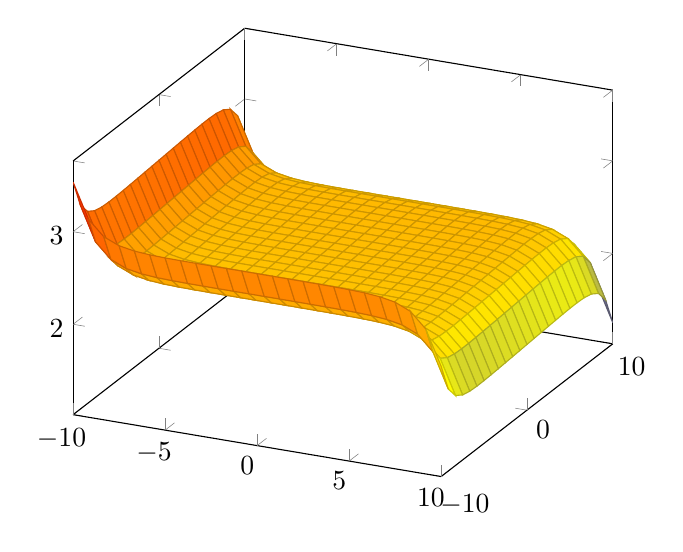
\begin{tikzpicture}
\begin{axis}
\addplot3[surf, domain=-10:10, y domain=-10:10]{0.4*cos(x)+0.4*sin(y)-0.00006*sinh(x)-0.00005*sinh(y)+2};
\end{axis}
\end{tikzpicture}
\end{center}

\begin{defi}[Fonction continue sur un ouvert de \(\R^2\)]
Soient \(\Omega\) un ouvert de \(\R^2\), \(f:\Omega\to\R\) et \(a\in\Omega\).

On dit que \(f\) est continue en \(a\) si on a : \[\quantifs{\forall\epsilon\in\Rps;\exists\delta\in\Rps;\forall x\in\Omega}\norme{x-a}\leq\delta\imp\abs{f\paren{x}-f\paren{a}}\leq\epsilon,\] \cad : \[\quantifs{\forall\epsilon\in\Rps;\exists\delta\in\Rps}f\paren{\Omega\inter\boulef{a}{\delta}}\subset\intervii{f\paren{a}-\epsilon}{f\paren{a}+\epsilon},\] \cad : \[\quantifs{\forall\epsilon\in\Rps;\exists\delta\in\Rps}\begin{dcases}
\boulef{a}{\delta}\subset\Omega \\
f\paren{\boulef{a}{\delta}}\subset\intervii{f\paren{a}-\epsilon}{f\paren{a}+\epsilon}
\end{dcases}\]

On dit que \(f\) est continue si elle est continue en tout de \(\Omega\).
\end{defi}

\begin{prop}
Soit \(\Omega\) un ouvert de \(\R^2\).

L'ensemble \(\ensclasse{0}{\Omega}{\R}\) des fonctions continues de \(\Omega\) dans \(\R\) est un sous-anneau de \(\F{\Omega}{\R}\).

Si \(f:\Omega\to\R\) et \(g:\Im f\to\R\) sont des fonctions continues alors \(g\rond f:\Omega\to\R\) est continue.

Si \(f:\Omega\to\R\) est continue alors l'ensemble \[\Omega\prim=f\inv\paren{\Rs}=\accol{x\in\Omega\tq f\paren{x}\not=0}\] est un ouvert de \(\R^2\) et la fonction \[\fonction{\dfrac{1}{f}}{\Omega\prim}{\R}{x}{\dfrac{1}{f\paren{x}}}\] est continue.
\end{prop}

\begin{dem}
\note{Exercice}
\end{dem}

\begin{exoex}
On pose : \[f:\paren{x,y}\mapsto x\qquad\text{et}\qquad g:\paren{x,y}\mapsto\Arctan\dfrac{y}{x}.\]

Pour chacune de ces fonctions, donner son ensemble de définition, dire si c'est un ouvert de \(\R^2\) et dire si la fonction est continue.
\end{exoex}

\begin{corr}
\(f\) est définie sur \(\R^2\) qui est un ouvert de \(\R^2\).

Soit \(\paren{a,b}\in\R^2\). Montrons que \(f\) est continue en \(\paren{a,b}\).

On a : \[\begin{aligned}
\quantifs{\forall\paren{x,y}\in\R^2}\abs{f\paren{x,y}-f\paren{a,b}}&=\abs{x-a} \\
&=\sqrt{\paren{x-a}^2} \\
&\leq\sqrt{\paren{x-a}^2+\paren{y-b}^2} \\
&=\norme{\paren{x,y}-\paren{a,b}}.
\end{aligned}\]

On a donc : \[\quantifs{\forall\epsilon\in\Rps;\exists\delta\in\Rps;\forall\paren{x,y}\in\R^2}\norme{\paren{x,y}-\paren{a,b}}\leq\delta\imp\abs{f\paren{x,y}-f\paren{a,b}}\leq\epsilon\] car \(\delta=\epsilon\) convient.

Donc \(f\) est continue.

\(g\) est définie sur \(\Rs\times\R\) qui est un ouvert de \(\R^2\).

De même que précédemment, \(\paren{x,y}\mapsto y\) est continue.

Donc \(\paren{x,y}\mapsto\dfrac{y}{x}\) est continue sur \(\Rs\times\R\).

Or \(\Arctan:\R\to\R\) est continue donc \(g\) est continue par composition.
\end{corr}

\section{Fonctions de classe \(\classe{1}\)}

\subsection{Développement limité d'ordre 1}

\begin{nota}
Soient \(\Omega\) un ouvert de \(\R^2\) contenant \(\paren{0,0}\) et \(g:\Omega\to\R\).

On dit que \(g\paren{x}\) est négligeable devant \(\norme{x}\) et on note \(g\paren{x}\underset{x\to\paren{0,0}}{=}o\paren{\norme{x}}\) si on a : \[\quantifs{\forall\epsilon\in\Rps;\exists\delta\in\Rps;\forall x\in\Omega}\norme{x}\leq\delta\imp\abs{g\paren{x}}\leq\epsilon\norme{x}.\]
\end{nota}

\begin{defi}
Soient \(\Omega\) un ouvert de \(\R^2\), \(f:\Omega\to\R\) et \(a=\paren{a_1,a_2}\in\Omega\).

On dit que \(f\) admet un développement limité à l'ordre 1 en \(a\) s'il existe \(\lambda,\mu\in\R\) tels que : \[f\paren{a_1+h_1,a_2+h_2}\underset{h=\paren{h_1,h_2}\to\paren{0,0}}{=}f\paren{a_1,a_2}+\lambda h_1+\mu h_2+o\paren{\norme{h}}.\]

Les réels \(\lambda\) et \(\mu\) sont alors uniques.
\end{defi}